\documentclass[tikz, border=10pt]{standalone}
\usepackage{tikz}
\usetikzlibrary{arrows.meta, positioning, fit, backgrounds}

\begin{document}
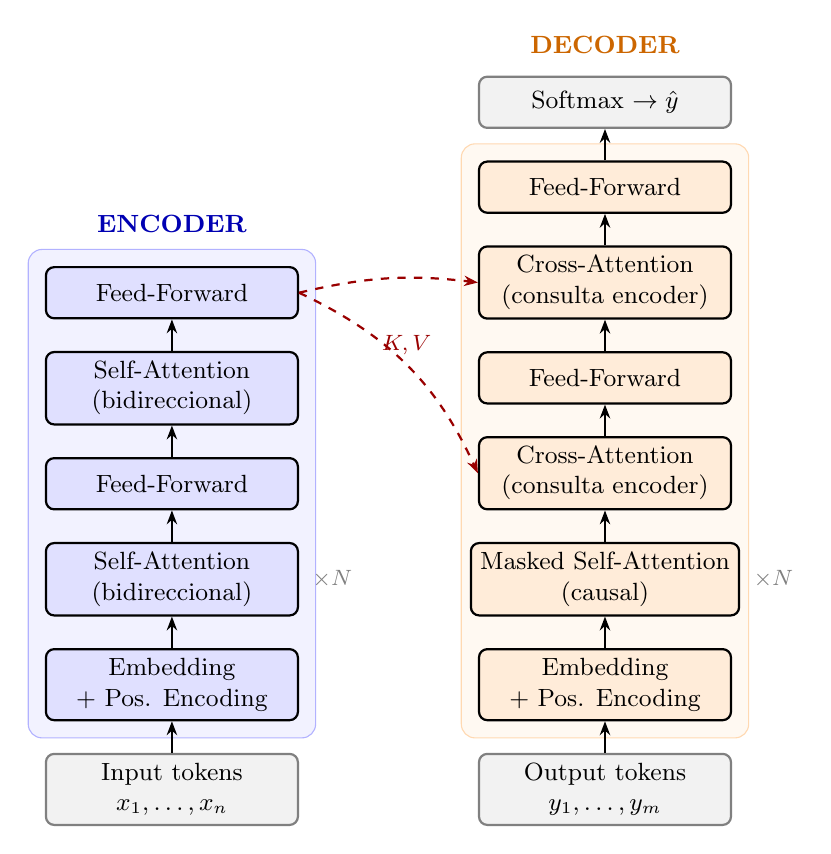
\begin{tikzpicture}[
    block/.style={draw, rounded corners=3pt, minimum width=3.2cm, minimum height=0.65cm,
                  thick, align=center, font=\small},
    enc/.style={block, fill=blue!12},
    dec/.style={block, fill=orange!15},
    io/.style={block, fill=gray!10, draw=gray},
    arr/.style={-{Stealth[length=5pt]}, thick},
    font=\small
]

% ---- ENCODER (left) ----
\node[io]                   (e_in)   at (0,0)   {Input tokens\\$x_1,\ldots,x_n$};
\node[enc, above=0.4 of e_in]  (e_emb)  {Embedding\\+ Pos. Encoding};
\node[enc, above=0.4 of e_emb] (e_sa)   {Self-Attention\\(bidireccional)};
\node[enc, above=0.4 of e_sa]  (e_ff)   {Feed-Forward};
\node[enc, above=0.4 of e_ff]  (e_sa2)  {Self-Attention\\(bidireccional)};
\node[enc, above=0.4 of e_sa2] (e_ff2)  {Feed-Forward};
\node[above=0.3 of e_ff2, font=\small\bfseries, blue!70!black] (elbl) {ENCODER};

\draw[arr] (e_in)  -- (e_emb);
\draw[arr] (e_emb) -- (e_sa);
\draw[arr] (e_sa)  -- (e_ff);
\draw[arr] (e_ff)  -- (e_sa2);
\draw[arr] (e_sa2) -- (e_ff2);

% Nx label
\node[right=0.05 of e_sa, font=\footnotesize, gray] {$\times N$};

% ---- DECODER (right) ----
\node[io]                   (d_in)   at (5.5,0)   {Output tokens\\$y_1,\ldots,y_m$};
\node[dec, above=0.4 of d_in]  (d_emb)  {Embedding\\+ Pos. Encoding};
\node[dec, above=0.4 of d_emb] (d_msa)  {Masked Self-Attention\\(causal)};
\node[dec, above=0.4 of d_msa] (d_ca)   {Cross-Attention\\(consulta encoder)};
\node[dec, above=0.4 of d_ca]  (d_ff)   {Feed-Forward};
\node[dec, above=0.4 of d_ff]  (d_ca2)  {Cross-Attention\\(consulta encoder)};
\node[dec, above=0.4 of d_ca2] (d_ff2)  {Feed-Forward};
\node[io,  above=0.4 of d_ff2] (d_out)  {Softmax $\to \hat{y}$};
\node[above=0.15 of d_out, font=\small\bfseries, orange!80!black] (dlbl) {DECODER};

\draw[arr] (d_in)  -- (d_emb);
\draw[arr] (d_emb) -- (d_msa);
\draw[arr] (d_msa) -- (d_ca);
\draw[arr] (d_ca)  -- (d_ff);
\draw[arr] (d_ff)  -- (d_ca2);
\draw[arr] (d_ca2) -- (d_ff2);
\draw[arr] (d_ff2) -- (d_out);

% Nx label decoder
\node[right=0.05 of d_msa, font=\footnotesize, gray] {$\times N$};

% ---- Cross-attention arrows from encoder to decoder ----
\draw[arr, dashed, red!60!black, bend left=20]
    (e_ff2.east) to node[above, font=\footnotesize, red!60!black]{$K,V$} (d_ca.west);
\draw[arr, dashed, red!60!black, bend left=10]
    (e_ff2.east) to (d_ca2.west);

% ---- Background boxes ----
\begin{pgfonlayer}{background}
    \node[fit=(e_emb)(e_ff2), fill=blue!5, draw=blue!30, rounded corners=5pt,
          inner sep=6pt] {};
    \node[fit=(d_emb)(d_ff2), fill=orange!5, draw=orange!30, rounded corners=5pt,
          inner sep=6pt] {};
\end{pgfonlayer}

\end{tikzpicture}
\end{document}
